\section{Platform and passive components}\label{sec:platform}

This chapter reports the Phase-A simulations of the individual SiN elements named in the proposal~\cite{proposal}, from the waveguide cross-section to the system-level behaviour of the optical phased array (OPA), and the error-budget links that follow from them.

\subsection{Scope and methods}\label{sec:platform-methods}

The waveguide platform is stoichiometric LPCVD Si$_3$N$_4$, 400~nm thick (the CoE-CPPICS limit), with 200 and 300~nm films as foundry alternatives, clad in SiO$_2$. Material dispersion is taken from Luke et al.~\cite{LUKE} and Malitson~\cite{MAL}, and the thermo-optic coefficients ($2.45\times10^{-5}$~/K for Si$_3$N$_4$, $1\times10^{-5}$~/K for SiO$_2$) from~\cite{TRC}. The working wavelengths are 894.6~nm (Raman addressing on the Cs D1 line) and 1064.4~nm (transport tweezers).

Each element is modelled with the cheapest method that captures its physics: (i) vector FEM mode solving (femwell 0.1.12, second-order N\'ed\'elec elements) for straight, bent, coupled and leaky guides; (ii) effective-index reduction with guided-mode eigenmode expansion for MMIs; (iii) scalar overlap with Gaussian fibre modes for edge couplers; (iv) 2D FDTD (MEEP 1.35, 40~px/\textmu m) for grating antennas, with the Si substrate included; (v) $2\times2$ transfer matrices with Monte Carlo sampling for switches; (vi) 2D thermal FEM for heaters; (vii) 1D scalar Fourier optics for the OPA (emitter near field, Fourier-plane slit, aplanatic objective); and (viii) an exact harmonic-oscillator result for transport heating. The mode, slab, MZI, OPA and transport models are checked against analytic limits or published examples (16 unit tests); the FDTD closes its energy balance to better than 0.5\%, and the heater result changes by 1.4\% when the domain is doubled.

The principal limits are as follows. The MMI and grating models are 2D. Edge-coupler numbers are mode overlaps without Fresnel or taper conversion loss. The OPA model is scalar and 1D along the steering axis, with an aberration-free objective. Sidewall scattering loss and fabrication roughness are not modelled. The AlN actuator is a single mechanical mode with assumed resonance frequency and quality factor. Every simulated value below is valid only within the regime simulated; the provenance of each input (proposal value, source, derived, design choice or recalled) is listed in Appendix~\ref{app:params}.

\subsection{Waveguide platform}\label{sec:platform-wg}

We choose the design width as the widest width on a 0.1~\textmu m grid for which (i) the TE1 mode is cut off or lies within 0.015 of the cladding index, and (ii) the TE0/TM0 effective-index splitting is at least 0.015. The second condition matters on the thick film: at 894.6~nm a $0.4\times0.4$~\textmu m$^2$ guide is polarisation-degenerate (TE0 = TM0 = 1.693), which would couple the polarisations in bends. Hence we use 0.5~\textmu m there. Table~\ref{tab:platform-modes} lists the resulting designs.

\begin{table}[htbp]\centering\small
\caption{Single-mode design guides (simulated, vector FEM). Here, $n_\mathrm{eff}$ and $n_g$ are the effective and group indices of TE0, $\mathrm{d}n_\mathrm{eff}/\mathrm{d}T$ is for uniform heating of core and cladding, and $R$ is the bend radius for less than 0.01~dB per $90^\circ$ bend.}
\label{tab:platform-modes}
\begin{tabular}{ccccccc}
\toprule
film & $\lambda$ & width & $n_\mathrm{eff}$ & $n_g$ & $\mathrm{d}n_\mathrm{eff}/\mathrm{d}T$ & $R$, TE / TM \\
(nm) & (nm) & (\textmu m) & & & ($10^{-5}$/K) & (\textmu m) \\
\midrule
400 & 1064.4 & 0.6 & 1.708 & 2.14 & 2.36 & 8 / 10 \\
400 & 894.6 & 0.5 & 1.745 & 2.17 & 2.41 & 6 / 6 \\
200 & 1064.4 & 0.9 & 1.613 & 1.98 & 2.02 & 20 / 60 \\
200 & 894.6 & 0.7 & 1.651 & 2.05 & 2.16 & 20 / 30 \\
\bottomrule
\end{tabular}
\end{table}

Substrate leakage on the 400~nm film is below $10^{-5}$~dB/cm for a buried oxide of 2~\textmu m or more at both wavelengths. On the 200~nm film at 1064.4~nm the oxide must be at least 3~\textmu m (TE leakage $7\times10^{-8}$~dB/cm); at 2~\textmu m, TM leaks 0.33~dB/cm. The coupling length of two 1064.4~nm guides on the 400~nm film is 1.8~mm at 1.6~\textmu m pitch and 29~mm at 2.1~\textmu m pitch, which sets how closely routing guides can run in parallel. At 1.4~W in one guide the peak in-guide intensity is 420~MW/cm$^2$ and the Kerr phase 0.05~rad/cm (with a Kerr index of $2.5\times10^{-19}$~m$^2$/W, recalled, to be verified).

The thick film confines both polarisations well. On 400~nm film the TM bend loss is only about ten times the TE loss at the same radius, hence bends cannot strip TM light. On 200~nm film at 1064.4~nm, in contrast, a 20~\textmu m bend radiates 1.5~dB per $90^\circ$ of TM against $5\times10^{-4}$~dB of TE, which makes a compact TM filter possible; at 894.6~nm the same film gives only 0.03~dB per $90^\circ$ of TM. This matters for the switch extinction (Sec.~\ref{sec:platform-switch}).

\subsection{Edge couplers and splitters}\label{sec:platform-couplers}

Inverse tapers on the 400~nm film reach a mode overlap of $-0.37$~dB with a 2.5~\textmu m lensed fibre at 1064.4~nm (150~nm tip, $\pm0.6$~\textmu m lateral tolerance at $-1$~dB) and $-0.48$~dB with HI1060 fibre (100~nm tip, $\pm1.55$~\textmu m). At 894.6~nm the best values are $-0.46$~dB (lensed) and $-1.1$~dB (PM780). The fibre mode-field diameters used (HI1060 6.2~\textmu m, PM780 5.3~\textmu m) are recalled, to be verified against datasheets. Several optima lie at the narrowest tip swept (100~nm), so narrower tips may do better if lithography allows. These overlaps exclude Fresnel and taper conversion loss and are therefore lower bounds on the 1 to 2~dB per facet assumed in the proposal. At 1.4~W through one 400~nm facet the intensity is 45~MW/cm$^2$; three input fibres keep it below 20~MW/cm$^2$. We have no CW facet-damage threshold for SiN at 1~\textmu m ([VALUE?]).

A 4~\textmu m wide $1\times2$ MMI has 0.044~dB excess loss at both wavelengths (lengths 14.8~\textmu m at 1064.4~nm and 17.7~\textmu m at 894.6~nm), so a 6-stage, 64-way tree costs 0.27~dB, against the ${\sim}1$~dB assumed. A symmetric $1\times2$ MMI is balanced by symmetry; imbalance arises only from asymmetric errors, 0.13~dB for a 20~nm lateral offset of the input guide. With $1\sigma$ errors of 10~nm (width), 5~nm (thickness) and 5~nm (offset), the $2\times2$ split ratio varies by 0.0024 (894.6~nm) and 0.0034 (1064.4~nm). Our first-pass 894.6~nm $2\times2$ design sits at 0.490 rather than 0.500; this offset is removable by redesign and is carried separately below.

\subsection{Switches, router and phase shifters}\label{sec:platform-switch}

The proposal asks for $\ge 50$~dB extinction at 894.6~nm. A single balanced MZI with a phase error $\delta$ has an extinction $\mathrm{ER} = -20\log_{10}(\delta/2)$, so 50~dB needs $\delta \le 6.3$~mrad. In practice the split-ratio spread of the MMIs dominates. Table~\ref{tab:platform-switch} and Fig.~\ref{fig:platform-extinction} compare three architectures with the simulated fabrication spread (0.0024) and a 0.5\% rms arm amplitude imbalance.

\begin{table}[htbp]\centering\small
\caption{Simulated MZI switch extinction at 894.6~nm (Monte Carlo, split-ratio spread 0.0024, arm amplitude imbalance 0.5\% rms). Here, $P$ is the fraction of devices reaching $\ge 50$~dB; ``trimmed'' means an input splitter trimmed to match the output coupler.}
\label{tab:platform-switch}
\begin{tabular}{lcccccc}
\toprule
& \multicolumn{3}{c}{phase error 3 mrad} & \multicolumn{3}{c}{phase error 10 mrad} \\
\cmidrule(lr){2-4}\cmidrule(lr){5-7}
Architecture & median & 5th pct & $P$ & median & 5th pct & $P$ \\
& (dB) & (dB) & & (dB) & (dB) & \\
\midrule
single MZI & 49.8 & 41.4 & 0.49 & 45.3 & 38.8 & 0.21 \\
single MZI, trimmed & 55.1 & 48.8 & 0.89 & 44.6 & 38.3 & 0.18 \\
two cascaded MZIs & 100 & 88 & 1.00 & 92 & 81 & 1.00 \\
\bottomrule
\end{tabular}
\end{table}

\begin{figure}[htbp]\centering
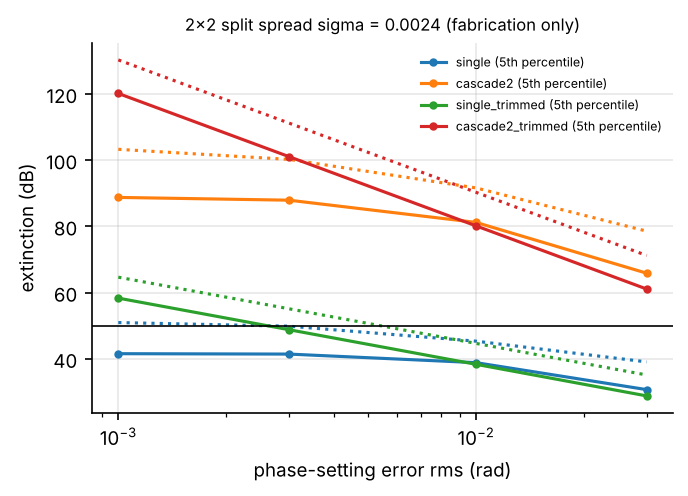
\includegraphics[width=0.7\linewidth]{m4_extinction.png}
\caption{Extinction of single, trimmed single, cascaded and trimmed cascaded MZI switches at 894.6~nm against the rms phase-setting error, from $2\times2$ transfer matrices with 4000 Monte Carlo trials per point. Solid lines with markers: 5th percentile; dotted lines: median. The $2\times2$ split ratio varies with the simulated fabrication spread $\sigma = 0.0024$ only (no design offset); arm amplitude imbalance 0.5\% rms. The horizontal line marks the 50~dB target.}
\label{fig:platform-extinction}
\end{figure}

A cascaded pair, as in~\cite{ZHAO}, reaches $\ge 50$~dB in every trial, with a 5th percentile of 88~dB. The 0.010 design offset of the first-pass $2\times2$ does not change this: it is shared by both couplers of an MZI, and two identical couplers still null exactly, so with the offset as a shifted mean the figures are unchanged ($P = 0.49$ for a single MZI, 88~dB for the cascade). An incoherent stray-light floor of $-70$~dB caps the cascade at 70~dB. For the AlN half-wave voltage at 894.6~nm, which we bracket between 84~V ($\lambda$-scaled from 74.7~V at 795~nm~\cite{ZHAO}) and 132~V (interpolated to 200~V at 1013~nm~\cite{ZHAO}), the 6.3~mrad limit of a single MZI requires driver noise below 0.17 to 0.27~V rms. The measured $V_\pi$ at 894.6~nm remains open ([VALUE?]).

Hence the binding constraints are polarisation and free-space crosstalk, not the interferometer. TM light is not nulled when the TE path is. For an input polarisation extinction of 20~dB, 50~dB at the output needs 24 to 30~dB of TM suppression after the chip; for 25~dB input, 19 to 25~dB. On 400~nm film bends cannot provide this (Sec.~\ref{sec:platform-wg}), hence a polariser in the free-space delivery path or a dedicated on-chip TE-pass element is required.

The settling of the switch is set by mechanical ringing of the AlN actuator, not by its 26~ns optical rise~\cite{ZHAO}. For an assumed single mode at $f_0 = 20$~MHz and $Q = 10$ ([VALUE?] for the real values), an unshaped step needs 0.98~\textmu s to reach $-50$~dB after switch-off. A two-impulse (ZV) shaper gives 24~ns, but 0.43~\textmu s with a 2\% error in $f_0$; a three-impulse (ZVD) shaper gives 49~ns with a 2\% error and 0.19~\textmu s with 5\%, at a 28~ns optical rise. Thus settling within 100~ns needs ZVD shaping with $f_0$ known to about 2\%.

The 16-output router (four stages of thermo-optically tuned MZI splitters) leaks at most $1.4\times10^{-3}$ into the worst unaddressed output (95th percentile) for a 30~mrad trim error, so with the cascaded output switch the idle-site extinction exceeds 110~dB (116~dB at 30~mrad). Its insertion loss is 5.0~dB, of which 3~dB is the assumed free-space delivery, so 16 sites at 20~\textmu W need about 1~mW at the input.

Two families of phase shifter serve different time scales. Thermo-optic shifters with a 2~\textmu m wide heater 2~\textmu m above the core need 84~mW for $\pi$ at 1064.4~nm (68~mW at 894.6~nm), with a 34~\textmu s rise and 16\% thermal crosstalk to a guide 10~\textmu m away. Isolation trenches reduce these to 54~mW and 2\%, and an additional undercut to 3~mW, at a 1.5~ms rise. The thermal conductivities and heat capacities in this model are recalled values, to be verified. Thermo-optic shifters suit slow router trims but not OPA updates at $\ge 100$~kHz. For the OPA, the PZT shifters of~\cite{MONT} ($V_\pi$ of 2.8~V at 532~nm, about 5.6~V at 1064.4~nm by wavelength scaling, 0.4~MHz bandwidth) settle in about 2~\textmu s, within a 5~\textmu s update period; their hysteresis is not known ([VALUE?]).

\subsection{System-level behaviour of the OPA}\label{sec:platform-opa}

\paragraph{Range and resolution.} The atom-plane field is a scaled copy of the slit-filtered OPA far field. The number of resolvable positions along the steering axis equals the channel number $N$, so the range at the atoms is $N\lambda/(4\,\mathrm{NA}\,F)$. Here, NA is the objective numerical aperture and $F$ the pupil fill. Table~\ref{tab:platform-field} gives the consequences at NA 0.5 and 1064.4~nm. At full fill, 64 channels steer over $\pm33$~\textmu m (17 sites at 4~\textmu m pitch), not $\pm100$~\textmu m, and cannot place more than about 15 tweezers on one row. More than 20 simultaneous tweezers on one row need 128 channels; at 0.75 fill they cover $\pm89$~\textmu m at 1.33 times the power per tweezer. Uniform channel amplitudes give 4.7\% first sidelobes along the steering axis; a Gaussian channel apodisation ($1/e^2$ at the aperture edge) lowers them to 0.9\% at a FWHM of 1.09~\textmu m. Section~\ref{sec:engine} builds on this count.

\begin{table}[htbp]\centering\small
\caption{Simulated steering field of the OPA (1D scalar Fourier optics, NA 0.5, 1064.4~nm). Here, the half-range is the usable one, in which the steered peak keeps at least half its on-axis value; ``sites'' is the number of 4~\textmu m sites on one row within it; and ``power'' is the relative power for equal depth.}
\label{tab:platform-field}
\begin{tabular}{cccccc}
\toprule
$N$ & fill $F$ & half-range (\textmu m) & sites & FWHM along $x$ (\textmu m) & power \\
\midrule
32 & 1.0 & 16 & 9 & 0.95 & 1.00 \\
64 & 1.0 & 33 & 17 & 0.95 & 1.00 \\
64 & 0.5 & 68 & 35 & 1.89 & 1.99 \\
128 & 1.0 & 67 & 33 & 0.94 & 1.00 \\
128 & 0.75 & 89 & 45 & 1.26 & 1.33 \\
256 & 1.0 & 134 & 67 & 0.94 & 1.00 \\
\bottomrule
\end{tabular}
\end{table}

\paragraph{Emitter type and pitch.} A Fourier-plane slit passes only the central diffraction zone, so the efficiency into it falls with emitter pitch: 0.65 at 1.5~\textmu m, 0.52 at 2~\textmu m and 0.34 at 3~\textmu m for the 0.6~\textmu m emitter guide (a wider emitter mode at the facet raises these, Sec.~\ref{sec:engine}). The minimum pitch is set by coupling between neighbouring emitters over their parallel length, for less than $-20$~dB power transfer: 1.46~\textmu m for an end-fire facet with an assumed 50~\textmu m parallel section, against 1.30, 1.56 and 1.82~\textmu m for gratings with 200, 100 and 50~nm etch (parallel lengths 20, 90 and 384~\textmu m). The gratings radiate 0.76, 0.72 and 0.68 upward at 8.9 to $10.0^\circ$, but their directionality oscillates with oxide thickness through the substrate reflection (0.42 to 0.76 over 2 to 4~\textmu m), the emission angle moves by $-0.10^\circ$/nm, and the 200~nm etch reflects 6\% back into the guide. Our choice of end-fire emitters is a compromise between two considerations. First, end-fire allows a dense pitch with short parallel sections, has no directionality loss and points independently of wavelength. However, it emits in plane and needs a relay to turn the beam towards the objective. The grating array becomes attractive only if a bottom reflector or two-layer grating is available.

\paragraph{Simultaneous tweezers by phase synthesis.} With weighted Gerchberg-Saxton alone ([REF?], recalled reference to be verified), light at untargeted lattice sites reaches 11 to 21\% of the tweezer intensity. A refinement that also penalises stray light and off-centre spots holds it at 3 to 7\%: for $N = 64$ with 8 or 12 tweezers the maximum stray is 0.056 and 0.053 and the maximum peak non-uniformity $(I_\mathrm{max}-I_\mathrm{min})/(I_\mathrm{max}+I_\mathrm{min})$ is 0.062 and 0.061; for $N = 128$ with 16 or 21 tweezers the stray is 0.054 and 0.057 and the non-uniformity 0.106. About 0.45 of the emitted power reaches the tweezers in all cases (four random target sets per case, one row along the steering axis). A 5.7\% stray at a static site corresponds to about 70~\textmu K under a 1.2~mK transport tweezer. This stray floor is one reason the steering engine of Section~\ref{sec:engine} avoids shared-aperture synthesis.

\paragraph{Phase accuracy.} For independent channel phase errors of rms $\sigma$, the position jitter at the atoms is $\sigma\sqrt{12/N}\,\lambda/(4\pi\,\mathrm{NA})$, which Monte Carlo reproduces to 2\%. Hence a 10~nm position error needs $\sigma \le 0.14$~rad at $N = 64$ (0.10~rad at 32, 0.19~rad at 128). Thus 8-bit phase resolution (7~mrad) is sufficient, and a PZT hysteresis error must stay below about 4\% of the applied phase at $N = 64$.

\paragraph{Update rate.} A tweezer moved by a staircase of OPA updates is excited because the staircase aliases the move spectrum to $|f_\mathrm{update}-f_\mathrm{trap}|$, where it can overlap the trap frequency. At the 1.2~mK transport depth the radial trap frequency is 84~kHz for $w_0 = 1.04$~\textmu m. As can be seen from Fig.~\ref{fig:platform-update}, a 100~kHz update then adds about 40 motional quanta to a 100~\textmu s, 4~\textmu m move and about 2,900 quanta to a 50~\textmu s move, against 0.005 and 0.2 for a smooth trajectory. At 200~kHz and above the staircase adds nothing measurable. Hence the $\ge 100$~kHz target of the proposal holds for 0.3~mK tweezers (42~kHz) but should read $\ge 200$~kHz for moves at 1.2~mK. Alternatively, lowering the depth to $\le 0.4$~mK during moves (48~kHz) with move times of $\ge 100$~\textmu s keeps 100~kHz: a 4~\textmu m move then adds 0.025 quanta (0.008 for a smooth trajectory).

\begin{figure}[htbp]\centering
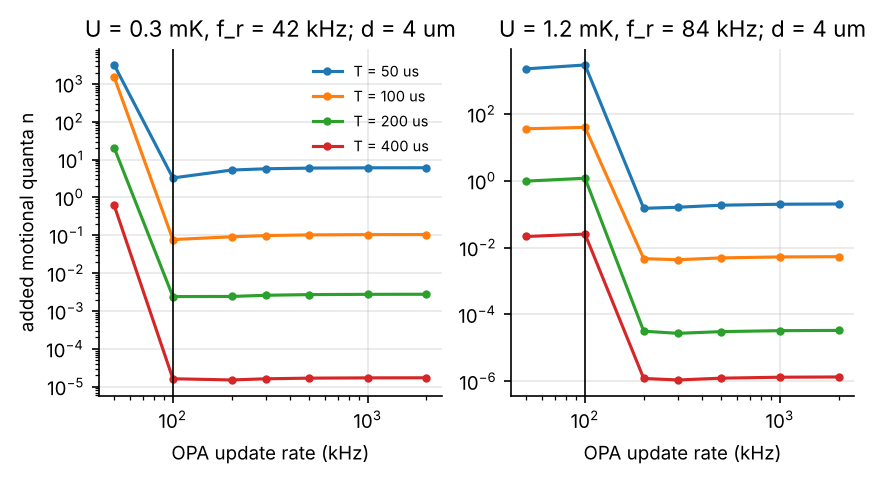
\includegraphics[width=0.85\linewidth]{m3_update_rate.png}
\caption{Motional quanta added to an atom by a 4~\textmu m OPA move against the update rate, for move durations $T$ of 50 to 400~\textmu s, at 0.3~mK ($f_r = 42$~kHz, left) and 1.2~mK ($f_r = 84$~kHz, right). Exact harmonic-oscillator result on the radial axis, atom initially in the ground state, minimum-jerk trajectory sampled and held at the update rate, $w_0 = 1.04$~\textmu m, polarisability 1160~a.u. The vertical line marks the 100~kHz target of the proposal. The curves are nearly flat from 200~kHz at 1.2~mK and from 100~kHz at 0.3~mK.}
\label{fig:platform-update}
\end{figure}

\paragraph{Loss budget.} For an end-fire OPA with $N = 128$, 21 tweezers and 2~\textmu m pitch, the chain from fibre to atoms is: edge coupler $-0.37$~dB, MMI tree $-0.27$~dB, propagation over 1~cm at 0.3~dB/cm (assumed) $-0.30$~dB, emitters with slit, pupil and synthesis $-3.43$~dB, and meta-objective transmission 0.7 (assumed) $-1.55$~dB, in total $-5.9$~dB. The grating case adds $-1.2$~dB of directionality ($-7.1$~dB for the best grating emitters). At 1.5~\textmu m pitch the slit term improves by about 1~dB. Against the ${\sim}10$~dB assumed in the proposal, the per-tweezer on-chip power falls from 66~mW to about 26~mW. This estimate excludes sidewall scattering.

\subsection{Phase-A error budget}\label{sec:platform-budget}

\paragraph{Idle-qubit error and trap depth.} The proposal's idle-qubit error for a switch of extinction ER is $(\pi^2/4)\,10^{-\mathrm{ER}/10}$, which gives $2.5\times10^{-5}$ at 50~dB when one Raman beam is addressed; we reproduce it. The proposal's trap depth is not reproduced: 6.6~mW in a Gaussian of $w_0 = 1.04$~\textmu m with a polarisability of 1160~a.u.\ gives 1.01~mK, not 1.2~mK; 1.2~mK needs 7.8~mW, or $w_0 = 0.96$~\textmu m. The OPA spot along the steering axis is 22\% brighter per watt than that Gaussian, which brings 6.6~mW to about 1.24~mK.

\paragraph{Addressing crosstalk.} Neighbour crosstalk of the 894.6~nm beams is set by the objective point-spread function, not by the chip. With a uniformly filled NA 0.5 pupil, the spot puts $1.0\times10^{-3}$ of its peak intensity on the 4~\textmu m neighbour, which gives a neighbour error of $2.5\times10^{-3}$, above the $10^{-3}$ budget. As can be seen from Fig.~\ref{fig:platform-crosstalk}, a Gaussian pupil fill truncated at 0.7 of the pupil radius brings this to $1.2\times10^{-4}$ (error $2.9\times10^{-4}$) at a spot FWHM of 1.13~\textmu m instead of 0.92~\textmu m. The model is aberration-free; a meta-objective with a Strehl ratio of 0.8 adds a halo that these figures do not include.

\begin{figure}[htbp]\centering
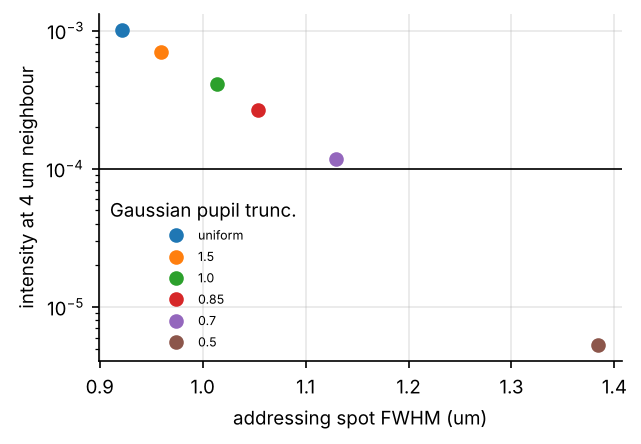
\includegraphics[width=0.6\linewidth]{m7_budget.png}
\caption{Intensity at the 4~\textmu m neighbour against the FWHM of the 894.6~nm addressing spot, for a uniform pupil and for Gaussian pupil fills truncated at 1.5, 1.0, 0.85, 0.7 and 0.5 of the pupil radius. Scalar Debye point-spread function, NA 0.5, aberration-free. The horizontal line marks $10^{-4}$.}
\label{fig:platform-crosstalk}
\end{figure}

\paragraph{Position and intensity noise.} The budget statement ``position noise $\le 10$~nm rms keeps transport survival $\ge 99\%$'' does not fix the heating rate, because heating depends on the noise spectral density at the trap frequency~\cite{OHARA}: $\dot{Q} = 4\pi^4 M\nu^4 S_x(\nu)$. Here, $M$ is the Cs mass (recalled, to be verified), $\nu$ the trap frequency and $S_x$ the position-noise spectral density. If 10~nm rms is white over 1~MHz, a 1.2~mK tweezer heats at about 7,700 quanta/s, about 0.8 quanta per 100~\textmu s move against a depth of about 300 quanta. Heating below 10 quanta/s needs $S_x(84~\mathrm{kHz}) \le 1.3\times10^{-25}$~m$^2$/Hz. In the same way, from $\Gamma = \pi^2\nu^2 S_I(2\nu)$~\cite{OHARA}, the relative intensity noise must satisfy $S_I(2\nu) \le 1.4\times10^{-11}$~/Hz at 1.2~mK for a parametric heating time of 1~s.

\paragraph{Power handling.} At 1.4~W into the input guide, with 0.3~dB/cm fully absorbed, the guide warms by 3.8~K and accrues 5.3~rad/cm of common-mode phase before the split. After the 64-way split each channel accrues at most 0.08~rad/cm, which the per-channel calibration absorbs.

\paragraph{Consequences for the specification.} The simulations imply six changes to the proposal's targets: (i) an OPA update rate of $\ge 200$~kHz for transport at 1.2~mK, or $\le 0.4$~mK during moves of $\ge 100$~\textmu s; (ii) a tweezer count tied to the channel count, with the steering field ($\pm33$~\textmu m at $N = 64$, $\pm68$~\textmu m at $N = 128$, $F = 1$) stated separately from the $\pm100$~\textmu m meta-objective field; (iii) about 6~dB (end-fire) to 7~dB (grating) of modelled chip and OPA loss, with 10~dB kept as the conservative value; (iv) position noise specified as $S_x(\nu_\mathrm{trap}) \le 1.3\times10^{-25}$~m$^2$/Hz, together with the 894.6~nm pupil apodisation needed for neighbour crosstalk $\le 10^{-4}$; (v) 7.8~mW, or the OPA spot, for 1.2~mK; and (vi) cascaded MZIs (or trimmed single MZIs with $\le 3$~mrad phase accuracy), an output polariser of $\ge 30$~dB on the 894.6~nm path, and ZVD-shaped drive for $\le 100$~ns settling. Item (ii) is superseded in its architectural part by the steering engine of Section~\ref{sec:engine}.
